
\textit{Ce développement présente l'algorithme de Peterson qui permet de résoudre le problème de l'exclusion mutuelle pour deux processus, le but étant de montrer la correction de l'algorithme. Il s'insère naturellement dans les leçons qui abordent la synchronisation et la gestion de ressources, comme les leçons \ref{L13}, \ref{L14} et \ref{L17}. Enfin, il peut illustrer la leçon \ref{L2} si le paradigme de programmation concurrente est abordé.}


\paragraph{Introduction.} Lorsqu'il y a une condition de concurrence, on veut que nos différents processus soient en exclusion mutuelle, c'est-à-dire qu'aucun des processus ne rentre dans leur section critique en même temps. Après une proposition non satisfaisante de Dekker (présentée par Dijkstra), Peterson a proposé une méthode élégante pour résoudre ce problème avec deux processus.


\begin{lstlisting}
#define FALSE 0
#define TRUE 1
#define N 2 / * nombre de processus * /
int turn;
int interested[N]; / * à qui le tour? * /

/ * on initialise les valeurs à 0 (FALSE) * /


void enter_region(int process) / * le processus est 0 ou 1 * /
{
	int other;  /* nombre de l'autre processus */
	other = 1 - process; /* l'opposé du processus */

	interested[process] = TRUE; /* on est intéressé */
	turn = other; /* on initialise le drapeau */

	 /* attente */
	while (turn == other && interested[other] == TRUE) ;
}

void leave_region(int process) 
{
	/* sortie de la région critique */	
	interested[process] = FALSE; 
}
\end{lstlisting}


\paragraph{Exclusion mutuelle.} 

\begin{proposition}
L'algorithme de Peterson vérifie la propriété d'exclusion mutuelle, c'est-à-dire deux processus ne rentrent jamais dans leurs sections critiques en même temps.
\end{proposition}
\begin{proof}
On raisonne par l'absurde. Supposons que le processus $0$ soit dans sa section critique, et le processus $1$ accède à la sienne. Ainsi, \texttt{enter\_region(0)} a terminé (le processus $0$ a réussi à rentrer dans sa section critique) et seulement après l'appel \texttt{enter\_region(1)} a terminé.

\begin{center}
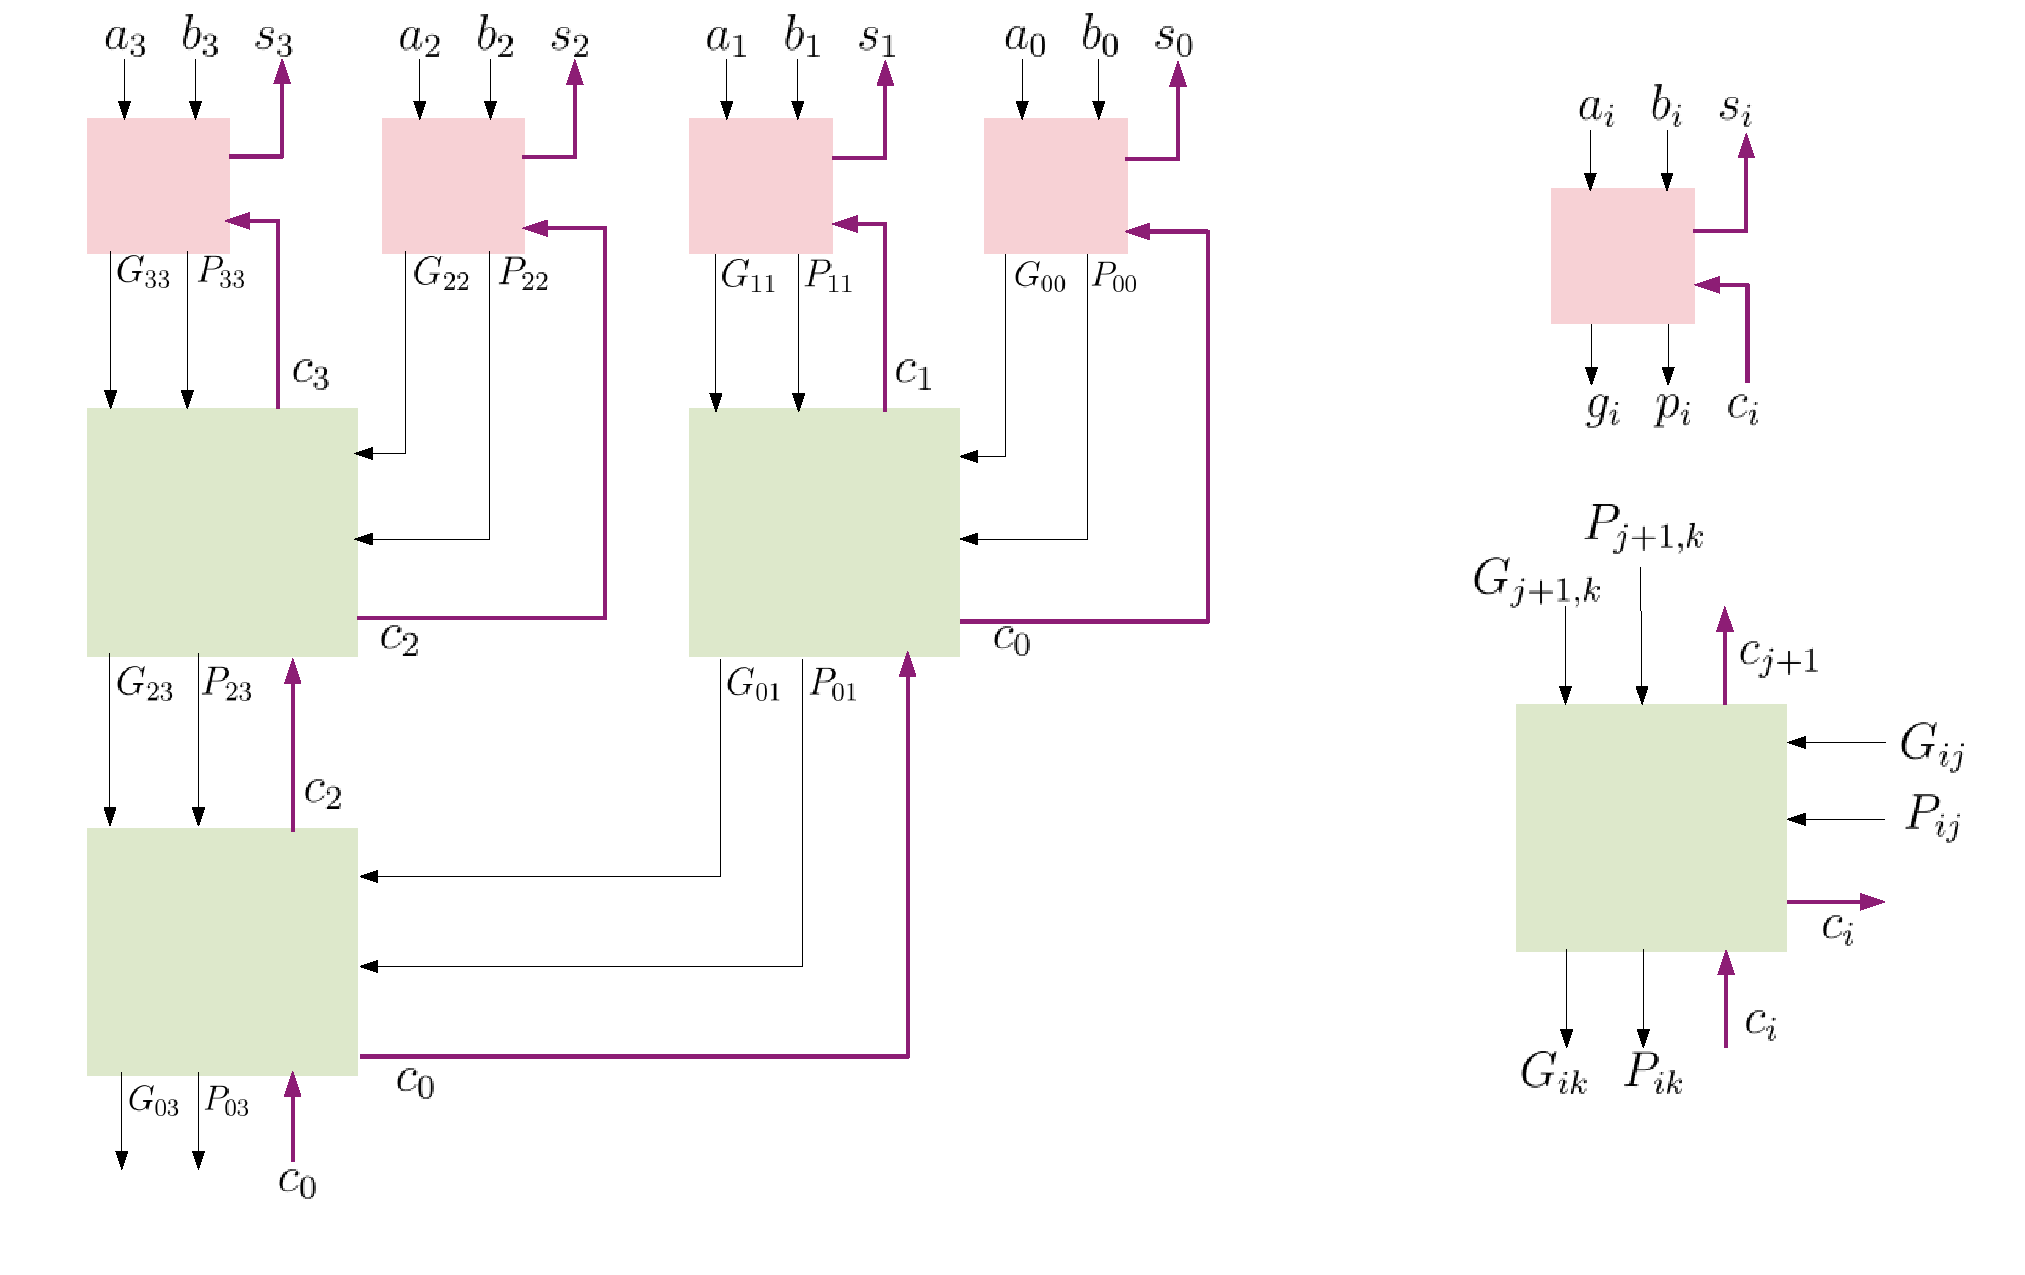
\includegraphics[scale=0.4]{Developpements/Peterson/schéma.pdf} 
\end{center}

\end{proof}

\paragraph{Exclusion mutuelle.}
\begin{proposition}
L'algorithme de Peterson ne provoque jamais d'interblocage, c'est-à-dire que si deux processus essaye d’accéder à leur section critique, au moins l'un des deux y arrive.
\end{proposition}

\begin{proof}
On raisonne par l'absurde, si les deux appels sont bloqués dans la boucle \texttt{while}, on a à la fois \texttt{turn == 1 } et \texttt{turn == 0 }.
\end{proof}


\paragraph{Absence de famine.}

\begin{proposition}
L'algorithme de Peterson assure l'absence de famine, c'est-à-dire que tout processus qui demande à rentrer en section critique y accède en temps fini, à condition que chaque processus reste un temps fini dans sa section critique.
\end{proposition}

\begin{proof}
Par l'absurde, si le processus $0$ lance son appel \texttt{enter\_region(0)} et reste bloque indéfiniment dans sa boucle \texttt{while} à partir de l'instant $t_0$. Donc pour tout temps $t\geq t_0$, on a \texttt{turn == 0} \texttt{interested[1] == TRUE}. Par la deuxième contrainte, on sait que le processus $1$ a appelé \texttt{entre\_region(1)}. De plus, le processus $1$ ne reste pas bloqué, puisque sinon il y aurait interblocage. Ainsi, $1$ entre en section critique et en sort en temps fini, il appelle alors {\tt leave\_region(1)}. À la fin de cet appel, on a {\tt intersted[1] == FALSE}. 
Il y a alors deux cas :
\begin{itemize}
\item si le processus $0$ reprend la main, alors on a une absurdité puisque {\tt intersted[1] == FALSE} ;
\item si le processus $1$ garde et appelle à nouveau {\tt enter\_region(1)}, alors il reste cette fois bloqué dans le {\tt while} puisqu'il est le dernier à avoir modifié {\tt turn}. Ainsi, lorsque le processus $0$ reprend la main, il est débloqué, ce qui est absurde aussi.
\end{itemize}
\end{proof}


\paragraph{Temps d'attente borné.}

\begin{proposition}
L'algorithme de Peterson assure une attente bornée, c'est-à-dire qu'un nombre borné de processeur peuvent passer avant lui lorsqu'il demande à entrer dans sa section critique.
\end{proposition}

\begin{proof}
Il suffit de reprendre la preuve précédente.
\end{proof}

